\section{Monte Carlo Simulation for Approximating Heat Content $Q_{\Omega}(t)$}\label{section:MC_heat_content}


  \subsection{Background \cite{jacobs2010stochastic}}
    \subsubsection{Stachasic Differential Equations (SDEs)}
      \begin{itemize}
        \item Stochastic process
        \item Brownian motion
      \end{itemize}
      
    \subsubsection{Connection Between SDEs and Heat Equation}
      \begin{itemize}
        \item Ito calculus
        \item Intepretating the heat equation by the probability density of particles undergoing Brownian motion
      \end{itemize}
      
  \subsection{A Special Case of Heat Content Calculation}

      \begin{itemize}
        \item Uniform initial tempretaure distribution in Eq.~\ref{eq:heat_content_integral_full}
          \par
          \begin{equation}\label{eq:uniform_initial_condition}
             f(\bm{s_0}) = \frac{1}{|\Omega|} 
          \end{equation}
          
          \begin{itemize}
           \item $|\Omega|$ is the area of the domain $\Omega$.
           \item Particles's initial positions are distributed uniformly in $\Omega$.
          \end{itemize}

        \item Intepretation of Eq.~\ref{eq:g}: observing all the Brownian particles unbiasedly.

        \item Probabilistic Intepretation of Heat Kernel $H_{\Omega}(\bm{s}, t | \bm{s_0})$: conditional probability density function of Brownian particles

        \item Probabilistic Interpretation of $Q_{\Omega}(t)$: Survival Probability $S_{\Omega}(\tau)$

          \begin{itemize}
           \item First passgae time $\tau$: the time taken by the particle to encounter the absorbing boudary $\partial \Omega$ from the initial position.
           \item Derivation of $S_{\Omega}(\tau)$ based on $H_{\Omega}(\bm{s}, t | \bm{s_0})$.
          \end{itemize}
    
      \end{itemize}


    \subsection{Monte Carlo Simulation (LRWs) for approximating $S_{\Omega}(\tau)$}

      \subsubsection{Monte Carlo Integration}
        \begin{itemize}
           \item Introduction
             \begin{itemize}
               \item Definition: utilizing the random sampling of a function to compute an estimate of its integral numerically \cite{hammersley1960monte}.
               \item Uniform Sampling Method
             \end{itemize}
           \item Given an initial position $\bm{s_0} \in \Omega$, approximating $H_{\Omega}(\bm{s}, t | \bm{s_0})$ by simulating the trajectories of a large number of particles by Lattice Random Walks (LRWs).
           \item Sampling a lager number of particles, whose initial sites are distributed uniformly within $\Omega$ to estimate $S_{\Omega}(\tau)$.
        \end{itemize}
        
     \subsubsection{Design LRWs in the $2-$ dimensional image}
       \begin{itemize}
           \item Initial condition: uniform distribution within $\Omega$, which is bounded by the border of the image and the edge of the target object.
           \item Boundary condition
             \begin{itemize}
               \item Perodic boundary condition the edges of the image.
               \par

               
                 \begin{figure}
                   \centering
                   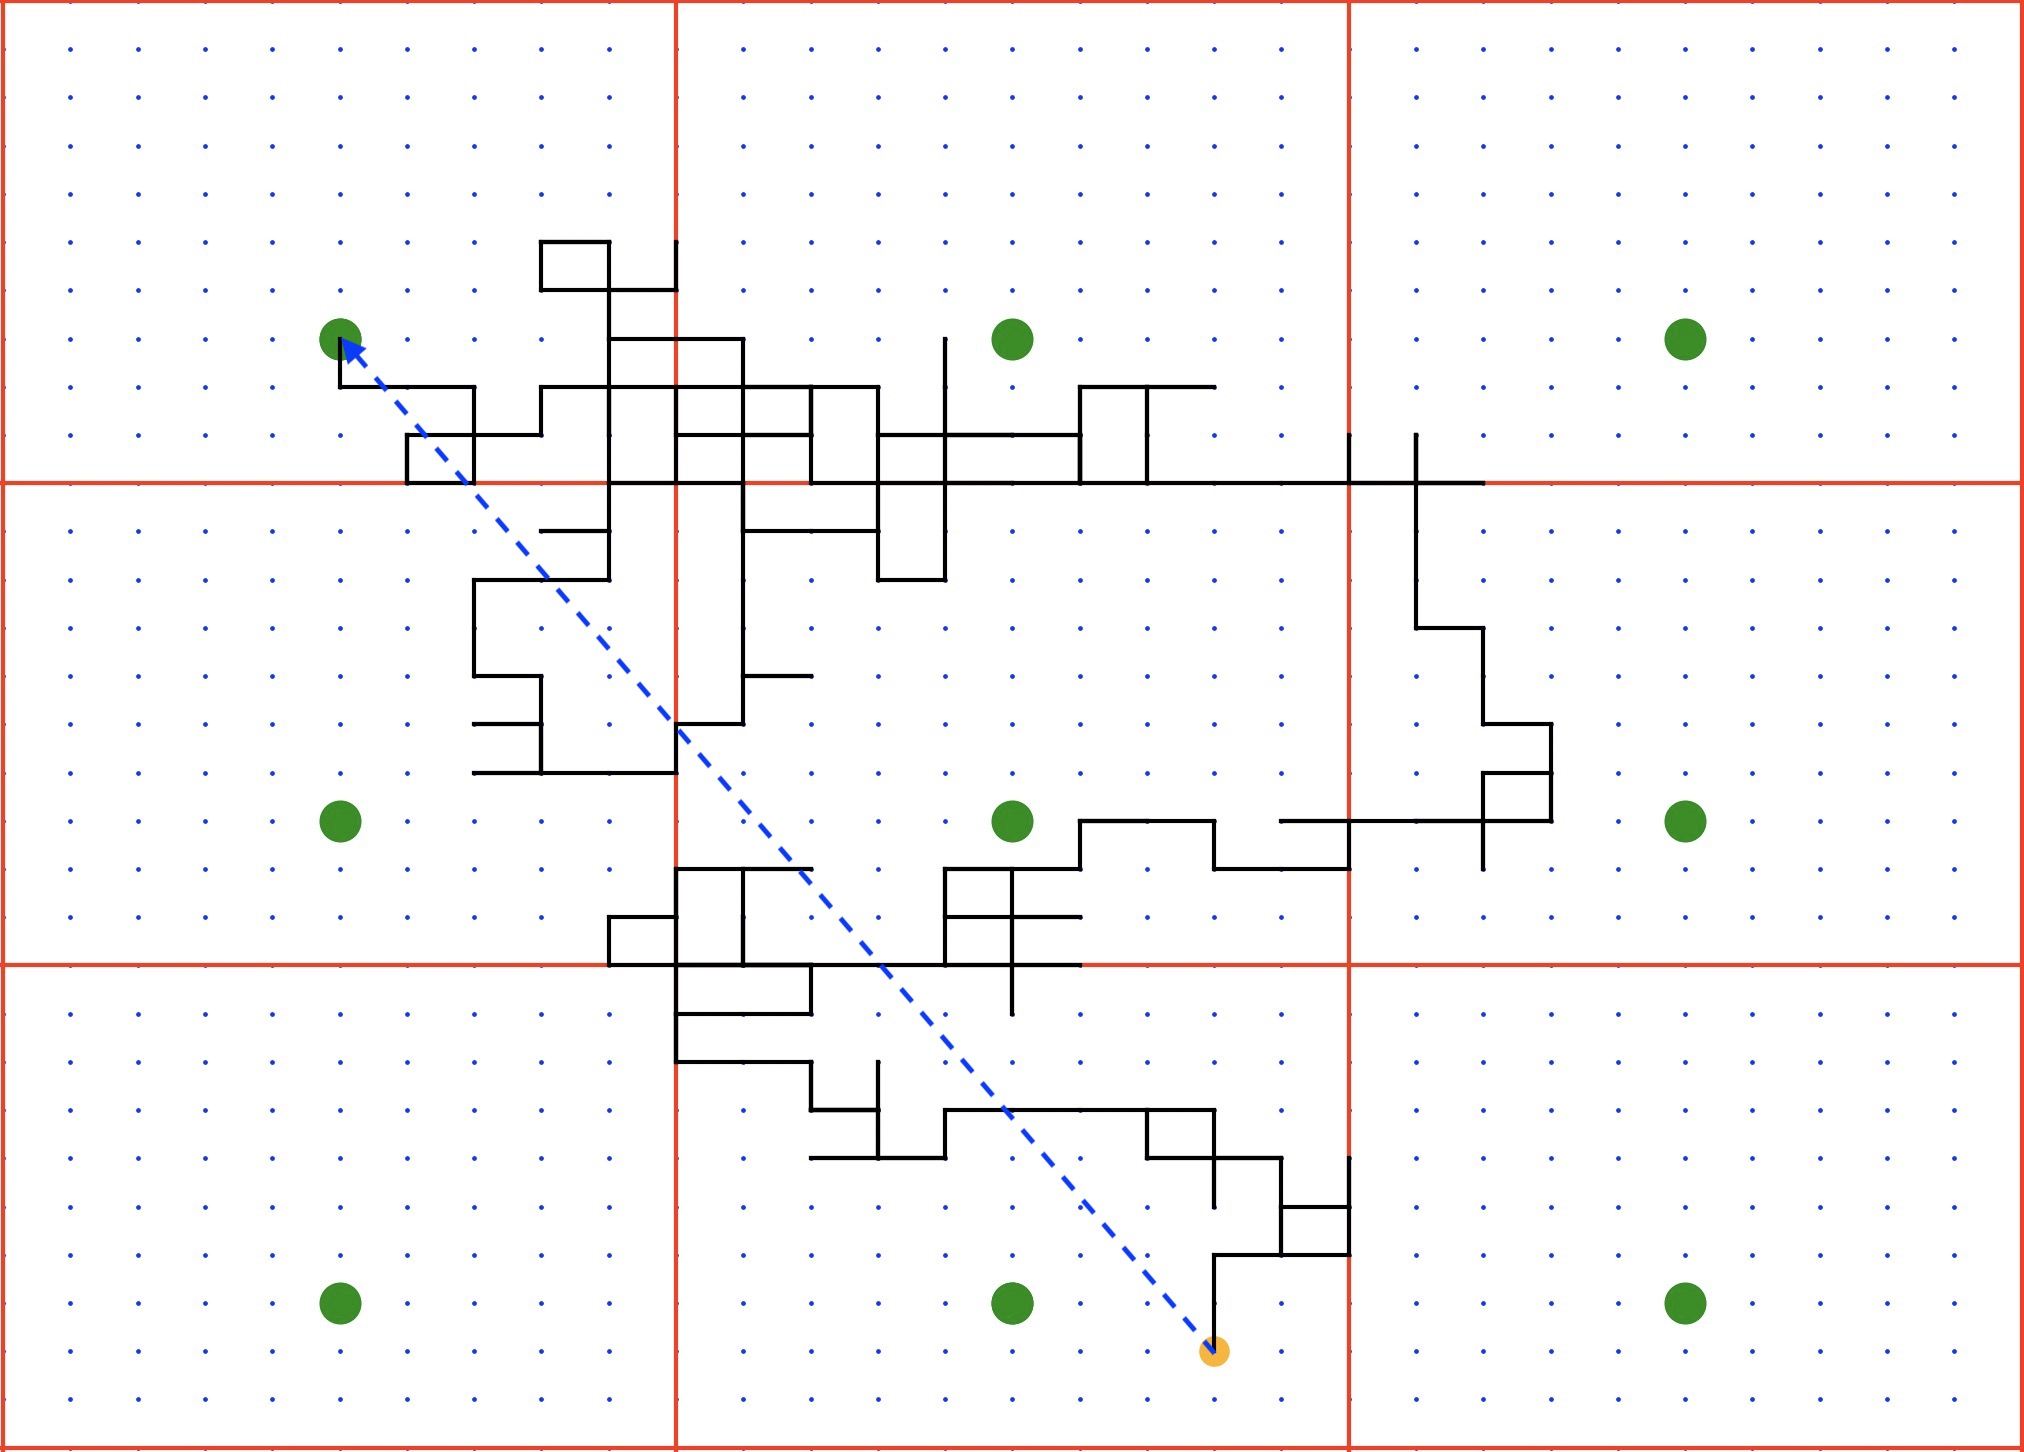
\includegraphics[width=\textwidth]{lrw_perodic_bc.png}
                   \caption{This plane is constructed by choosing a
                     primitive cell with four red sides and a green
                     point and replicating it infinitely to tile the
                     whole $2-$ dimensional space. Moreover, there has
                     no overlaps and voids between copies of the
                     cell. A particle initially started LRWs from the
                     orange site and be absorbed by any of the green
                     points.  To ensure smoothness and consistency, if
                     the particle leaves the cell through one edge, it
                     will appear in the adjacent cell with the same
                     velocity. The black line segments show the
                     particle's random trajectories, and the length of
                     the blue dotted arrow is defined as its
                     displacement.}
                   \label{fig:pbc_lrws}
                 \end{figure}


                 In this thesis, periodic boundary conditions (PBCs)
                 are employed to minimize the influence of images'
                 edges. Fig.~\ref{fig:pbc_lrws} is a simplest example
                 of implementing PBCs in the Euclidean plane $E^2$ and
                 tracks the trajectory of a particle undergoing LRWs.


               
               \item Absorbing boundary condition on the boundary of the target shape.
             \end{itemize}
       \end{itemize}
       
        

      \subsubsection{Sample Size Determination - Dvoretzky–Kiefer–Wolfowitz (DKW) inequality \cite{dvoretzky1956asymptotic}}

      \begin{itemize}
        \item Mathematical formula and interpretation
        \item Strengths
          \begin{itemize}
            \item Distribution-free
            \item Sample size calculation does not depend on 
              \begin{itemize}
                \item Domain shape and size
                \item Target geometry
                \item B.C.s
              \end{itemize}
          \end{itemize}
      \end{itemize}



      \subsubsection{Output Analysis}

        \begin{itemize}
          \item Kaplan-Meier Estimator \cite{kaplan1958nonparametric} \cite{aalen2008survival}\cite{cameron_davidson_pilon_2021_4505728}
          \item Confidence Interval \cite{greenwoodnatural} \cite{hosmer2011applied} \cite{kalbfleisch2011statistical}\cite{sawyer2003greenwood}
          \item Two-Sample Statistical Tests (weighted logrank tests) \cite{custodio2007diagnostics} \cite{agarwal2012statistics} \cite{karadeniz2017examining} \cite{leton2001equivalence} \cite{etikan2017kaplan} \cite{harrington1982class}
            \begin{itemize}
              \item Wilcoxon
              \item Tarone-Ware
              \item Peto
              \item Fleming-Harrington
            \end{itemize}
            
        \end{itemize}


        
      
      
    
      
